
\section{Introduction}
Deep Neural Networks (DNNs) have encountered great challenges when involving the applications \cite{krizhevsky2017imagenet,wang2021survey} on resource-constrained devices, owing to the increasing demands for computing and storage resources. Network quantization \cite{lin2016fixed,jacob2018quantization}, which reduces the model size and energy consumption by mapping the floating-point weighs and activations to low-bit ones, is a promising approach to improve the efficiency of DNNs for model compression \cite{han2015deep,qian2021diversifying}. Quantization methods generally dedicate themselves to recovering the \emph{performance drop} originating with the quantization errors, which involves fine-tuning or calibration operations with the original training data.






\begin{figure}[t]
\centering
%\setlength{\abovecaptionskip}{0.12cm}
\setlength{\belowcaptionskip}{-0.35cm}
\includegraphics[width=1.0\columnwidth]{previous_drawback.pdf}
\caption{Existing work, \emph{e.g.}, GDFQ \cite{xu2020generative} (the \textcolor[RGB]{30,118,180}{blue}) and Qimera \cite{choi2021qimera} (the \textcolor[RGB]{255,127,14}{orange}), suffers from a non-ignorable accuracy loss, as they fail to consider the sample adaptability.
Our AdaSG (the \textcolor[RGB]{44,160,44}{green}) generates the sample with desirable adaptability to maximally recover the performance of Q with varied bit widths, such as (a) 3-bit and (b) 5-bit precision. The observations are from ResNet-18 on ImageNet.  }
\label{drawback}
\end{figure}





However, in many real-world scenes, such as medical and military fields, the original data may not be accessible due to privacy and security issues.
Fortunately, recently proposed data-free quantization (DFQ), a potential method to quantize models without accessing the original data, aims to synthesize meaningful fake samples instead, which improves quantized network (Q) by knowledge distillation \cite{hinton2015distilling,qian2022switchable}  against the pre-trained full-precision model (P).
%The early work \cite{cai2020zeroq,zhang2021diversifying} optimized the random noise to synthesize samples by matching the batch normalization statistics of the synthetic data and real data based on full-precision model.
Among the prior researches \cite{cai2020zeroq,zhang2021diversifying}, the generative fashions \cite{xu2020generative,choi2021qimera,zhu2021autorecon} have recently attracted increasing attention, owing to their superior performance. The generative model is introduced as a generator (G) to capture the distribution of the original data from P for better fake samples, where P is regarded as the discriminator to guide the generation process . For example, Qimera \cite{choi2021qimera} generated boundary supporting samples to reduce the gap between the synthetic and real data.
Nevertheless, \emph{there still remains a non-ignorable performance loss when encountering various bit-width settings}. The reasons may lie in several aspects:
\begin{itemize}
    \item[(1)] Due to the limited capacity of the generator, the generated sample with incomplete distribution is impossible to fully recover the original dataset, so that  it is a crucial criterion: is the sample \emph{beneficial} or \emph{adversarial} over the learning process of Q? However, in the existing arts, the generated sample customized for P, can't always benefit Q in varied bit-width settings (\emph{e.g.}, 3-bit or 5-bit precision, refer to (2)(3)), where only limited information from P can be utilized to recover Q.
    \item[(2)] In 3-bit precision, Q often suffers from a sharp accuracy drop compared to P due to large quantization error, leading to its poor learning ability. Under such case, the generated sample by G may bring an unexpected large \emph{disagreement} between the predictions of P and Q, which makes the optimization loss too large to converge, resulting in no improvement; see the \textcolor[RGB]{255,127,14}{orange} flat curve in Fig.\ref{drawback}(a).
    \item[(3)] In 5-bit precision, Q still possesses comparable recognition ability with P due to a small accuracy drop. Under such case, most of the generated samples by G, for which Q and P give similar predictions (\emph{i.e.}, reach an \emph{agreement}), may not benefit Q. However, under the constraint of the optimization loss, Q receives no improvement, even impairment; see the \textcolor[RGB]{30,118,180}{blue} curve (Epoch 0-50) in Fig.\ref{drawback}(b).
\end{itemize}






\noindent Based on the above, the existing approaches fail to consider the \emph{sample adaptability}, \emph{i.e.}, beneficial or adversarial over the calibration process of Q, to Q with varied bit widths during the sample generation process from G, where Q is independent of the generation process; see Fig.\ref{knowledge_medium}(a). For example, for (2), the sample with large adaptability may be one with small disagreement between P and Q; while for (3), it may be one with large disagreement. The above naturally elicits the following basic questions: \emph{how to measure and exploit the sample adaptability to quantized network under varied bit-width scenarios? how to generate the sample with desirable adaptability to benefit the quantized network?}




\begin{figure}[t]
%\setlength{\abovecaptionskip}{0.12cm}
\setlength{\belowcaptionskip}{-0.35cm}
\centering
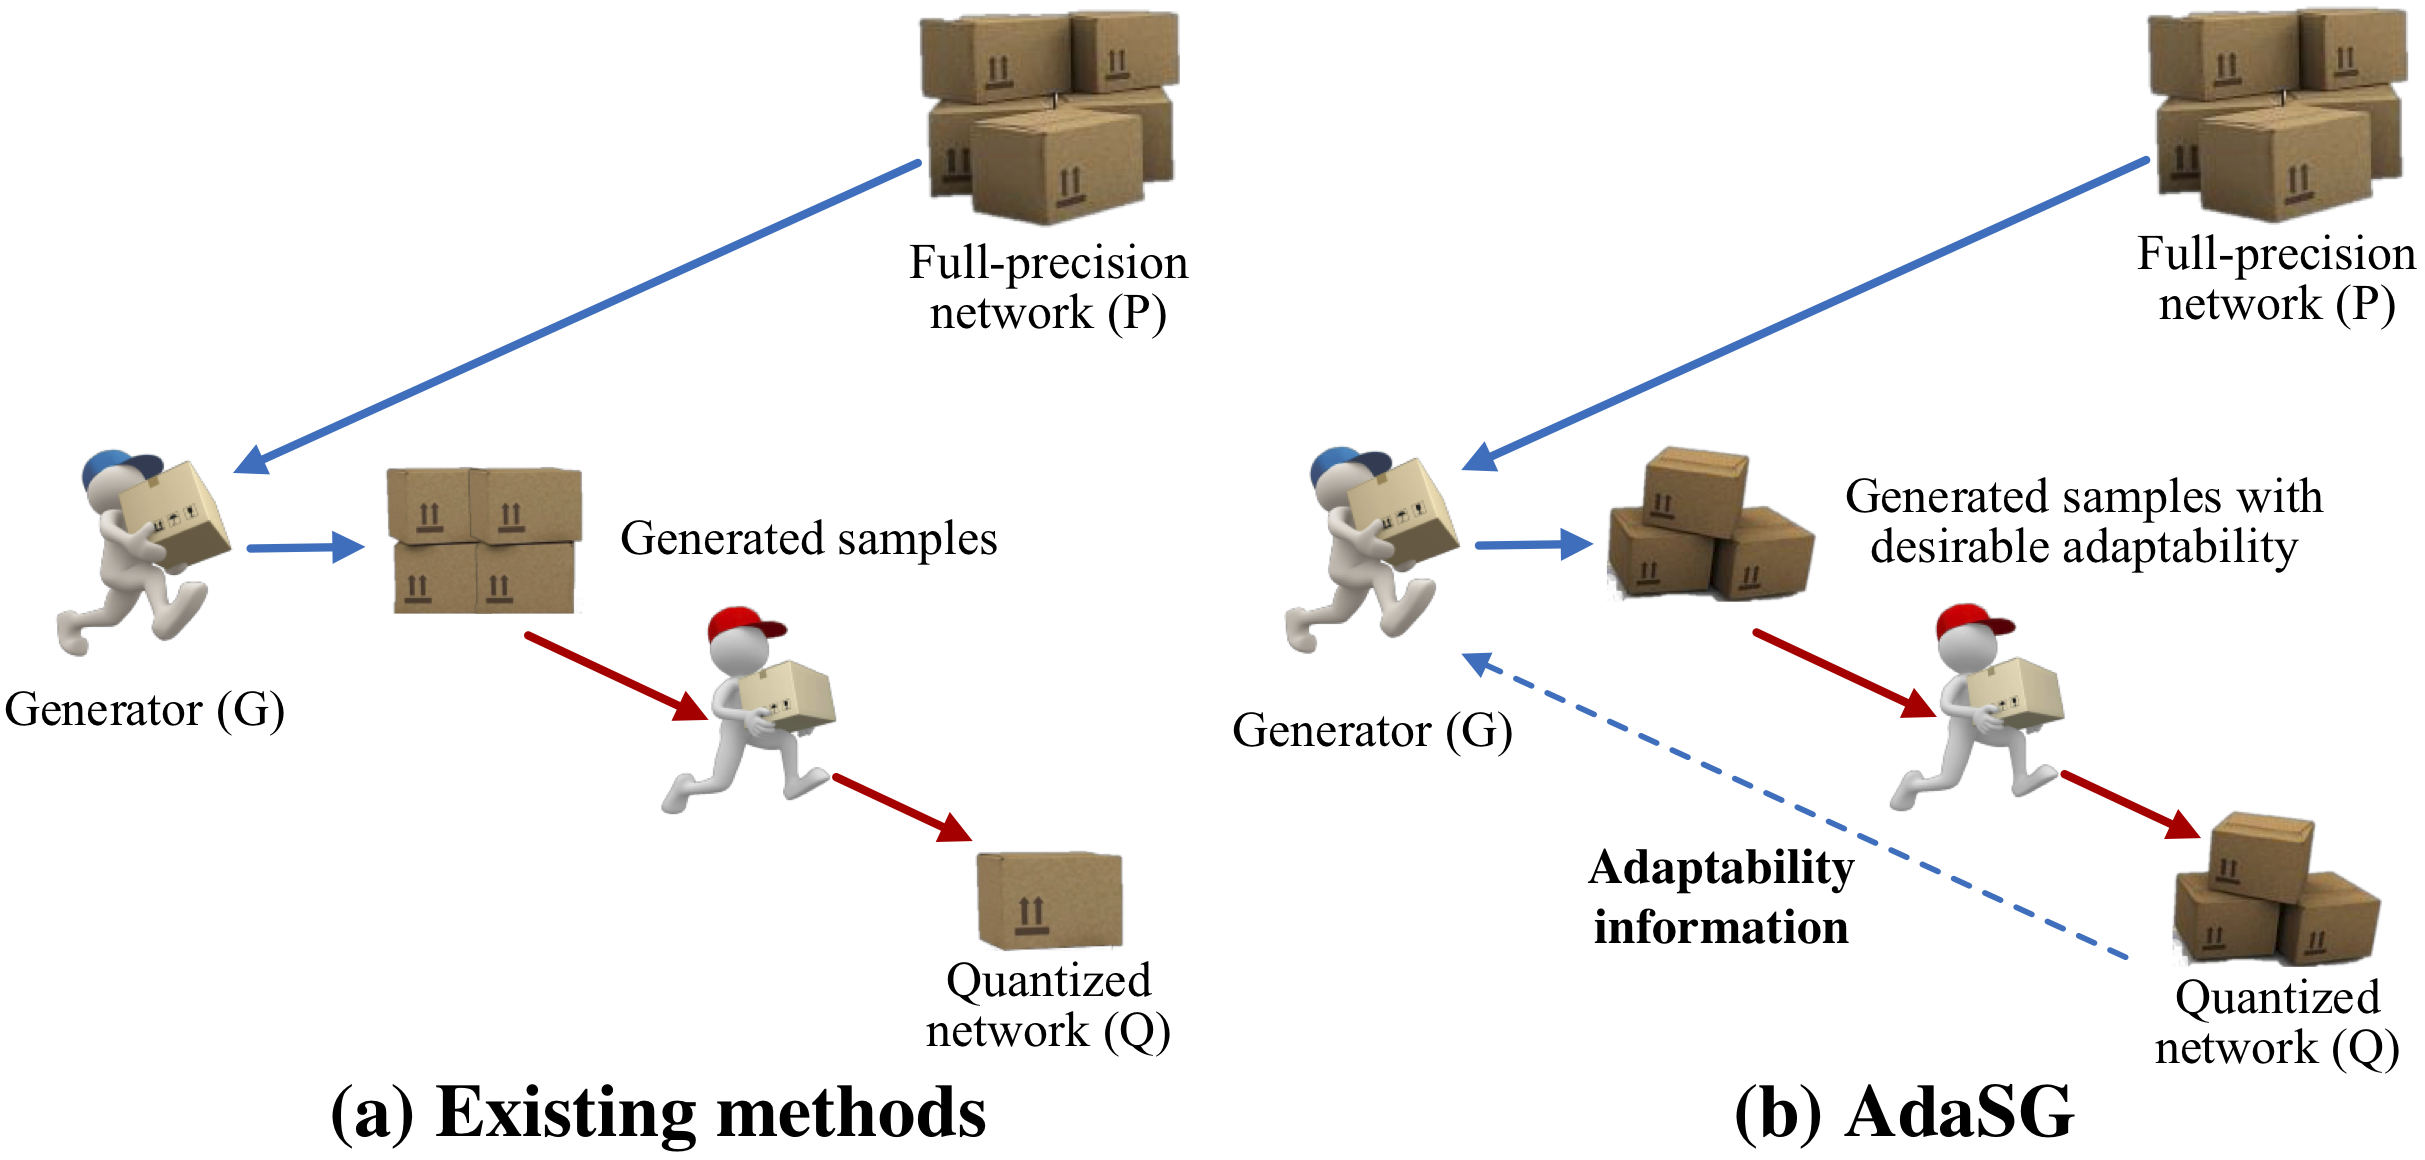
\includegraphics[width=1.0\columnwidth]{knowledge_medium.png}
\caption{Unlike the existing arts (a), our AdaSG (b) aims to generate the sample with desirable adaptability from G, \emph{i.e.}, the dependence of generated sample on Q, to maximally benefit Q with varied bit widths.}
\label{knowledge_medium}
\end{figure}









%Intuitively, we view the sample adaptability as the amount of the knowledge is successfully transferred from full-precision to quantized network.
To answer the above questions, we consider to generate the sample with large adaptability to Q by taking Q into account during the generation process; see Fig.\ref{knowledge_medium}(b).
%Specifically, the generator (G) generates the sample by exploiting the distribution from full-precision network and the sample adaptability to quantized network, while the quantized network learns from the generated samples with desirable adaptability. Accordingly, \emph{the more information carried in the sample is exploited to improve the quantized network in varied bit-width situations, the more desirable the sample adaptability is}; see Fig.\ref{knowledge_medium}(b).
Specifically, G aims to generate the sample with \emph{large} adaptability, which essentially \emph{maximizes} the reward for G, by enlarging the disagreement between P and Q, to benefit Q; while Q is calibrated to improve itself by exploiting the sample with large adaptability. It is apparent that such sample adaptability will not be large to Q after Q is refined; in other words, such process of benefiting Q leads to \emph{decreasing} the sample adaptability, which essentially \emph{minimizes} the loss for Q, and is adversarial to maximizing the reward goal for G. Based on the above, we rethink date-free quantization process and formulate it as a zero-sum game \cite{li2022policy,zhang2022no} between two players (an adversarial game process where one player's reward is the other's loss while their sum is zero) --- a generator and a quantized network; and we further propose an \textbf{Ada}ptability-aware \textbf{S}ample \textbf{G}eneration (AdaSG) method.
Technically, we specify it via a dynamic maximization-vs-minimization game process anchored on sample adaptability, and defined as:
\begin{equation}
\mathop{min}_{\theta_q\in \Theta_q} \mathop{max}_{\theta_g\in \Theta_g} \  \mathcal{R}(\theta_g,\theta_q),
\label{min_max_s_intro}
\end{equation}
where G and Q are parametrized by $\theta_g\in \Theta_g$ and $\theta_q\in \Theta_q$, respectively.
The optimization of Eq.(\ref{min_max_s_intro}) consists of  fixing $\theta_q$, and updating $\theta_g$ to the optimal $\theta_g^{'}$ for \textit{maximizing } $\mathcal{R}(\theta_g,\theta_q)$; while alternatively fixing $\theta_g^{'}$, and updating $\theta_q$ to the optimal $\theta_q^{'}$ for \textit{minimizing} $\mathcal{R}(\theta_g^{'},\theta_q)$.
%To promote the stationarity of the DFQ game \cite{zhang2022no}, that is, the knowledge carried in the sample can be ideally exploited to improve the quantized network, we introduce the notion of \emph{Balance Gap} (BG, see Definition 1 for details) as a measure, where BG tending to zero corresponds to the more desirable sample adaptability.
%Hence, BG is formulated as the difference of the objective function $R$ between the last and current iteration, in terms of the non-stationarity of zero-sum game \cite{zhang2022no}. Thus, whenever the DFQ game attains a stationarity point, BG will tend to zero, indicating that the knowledge contained in the synthetic samples is ideally digested to improve the quantized network.
%synthesize the satisfactory sample with a generative model for the quantized network in various bit-width situations.
Specifically, the maximization process exploits the sample adaptability to Q upon P to generate two types of samples: disagreement (\emph{i.e.}, P can predict correctly but Q not) and agreement samples (\emph{i.e.}, P and Q have the same prediction), such sample adaptability is further reduced by the minimization process after calibrating Q for performance recovery. To achieve the stationarity to maximally benefit Q,
the Balance Gap (BG) for the adaptability of the generated samples within the game process is defined to set up such a stationary objective to balance the maximization versus minimization process.
We remark that AdaSG is essentially an \emph{adversarial} game governed by the sample adaptability, which is fundamentally orthogonal to the existing arts that improve Q by transferring knowledge from P to Q.
One recent study \cite{liu2021zero} generates adversarial samples via G, by maximizing the gap between P and Q, and minimizing their gap to benefit Q for calibration.  However, it fails to consider the sample adaptability to Q, hence suffers from the non-ideal generated samples. Besides, they focus primarily on the adversarial sample generation rather than adversarial game process perspective for AdaSG to generate the samples with desirable adaptability.
The theoretical analysis and empirical studies validate the superiority of AdaSG to the state-of-the-arts.





%As a byproduct, we devise a boundary constraint on the sample adaptability to prevent the generation of the extreme samples.
%For the \emph{expanding} stage, to endow AdaSG with desirable adaptability to varied quantized networks, we push forward the coordination between two types of generated samples: namely \emph{disagreement sample} as hard sample --- P can predict correctly but Q not, and \emph{agreement sample} as easy sample --- P and Q have the same prediction.  For the \emph{shrinking} stage, the generated sample with ideal adaptability is utilized to calibrate the quantized network for the performance recovery.  The game between the expanding and shrinking offers a driving force for the DFQ process.





%Besides, an alternative method proposed by \cite{liu2021zero} is to generate adversarial samples by considering both full-precision and quantized model, which, however, often causes the generation of unexpected (out of distribution) samples, making the adversarial learning process be at a risk of collapse, thus the adversarial sample also lacks the adaptability.





%In contrast to the above, the focus of this paper lies in that, the synthetic sample is customized to meet the requirements of quantized network in various bit-width situations, which actually plays a role as a medium of knowledge transfer from full-precision to quantized network. This provides the guarantees that the knowledge contained in synthetic samples can be ideally transferred to improve the quantized network.


%These issues urge us to think deeply about how to boost the adaptability of synthetic samples to various bit-width situations.


%To address the above, how to enhance the adaptability of synthetic samples to different bit-width settings during the fine-tuning or calibration process remains an open question.






















